\chapter{Testing}
\label{chap:testing}

This chapter describes the testing approaches we used to ensure our habit-tracking application is reliable and working as expected. Throughout our development, we combined automated testing with targeted manual tests for cross-platform validation. While our automated coverage is high, our critical reflection reveals areas where we could have improved our quality assurance process.

\section{Approach and tools} \label{sect:testing:approach}

\subsection{Automated Testing}

We relied heavily on automated testing to make sure our features worked as expected. Each suite checks how the component renders, responds to user actions (e.g., button presses), and triggers any side effects. This approach helps us confirm that our UI logic, data calls, and component behaviours work as intended.

\paragraph{Tools Used} \begin{itemize} \item \textbf{Jest}: Our main test runner, responsible for executing the test suites. \item \textbf{React Native Testing Library}: Lets us simulate user interactions (like tapping buttons or typing text). \item \textbf{Some examples of our Mocking Techniques}: \begin{itemize} \item{AsyncStorage}: Replaces native storage calls so tests don’t fail on missing native modules. \item{Fetch}: Fakes server API calls, which means our tests do not depend on a real network. \item {Expo Router and ThemeContext:}
We replace real navigation and theming with simple "fake" versions. This way, our tests focus only on the component’s behavior, rather than on actual screen transitions or styles. \item {Victory Charts}: This library uses SVG (Scalable Vector Graphics) to draw charts. In our tests, we swap the real chart components for simpler “mocks.” This means the charts don’t actually get rendered, and our tests run faster with fewer errors. For example, in \texttt{BuildHabitGraph.test.tsx}, we check that the chart component receives the right data without drawing any real SVG. \end{itemize} \end{itemize}


\paragraph{Location of Automated Tests}\mbox{}\\

We keep our tests in the \texttt{client/src/components/\_\_tests\_\_} folder, and we name each file after the component it tests. For example:

\begin{itemize} \item \texttt{BuildHabitGraph.test.tsx}\item \texttt{WeeklyCalendar.test.tsx} \item \texttt{SettingsPage.test.tsx} \end{itemize}

This structure makes it easy to locate each test and ensures that test code remains closely tied to its corresponding component.

One critical reflection is that we did not integrate automated testing as thoroughly as we had hoped during development. Although we did test throughout the entire project, many tests were only added later in the project, which in hindsight left some functionalities untested for longer than we would have liked.

\subsection{Black-Box Testing Techniques}
Our automated tests followed key black-box testing principles. We focused on checking how the app responds to user actions and inputs, without relying on internal implementation details.

\begin{itemize}

\item \textbf{Boundary Value Analysis:}
In \texttt{HabitPanel.test.tsx}, we tested date-related edge cases. For example, confirming that users cannot open the progress dialog for future dates. These tests helped ensure the app prevents invalid actions outside the allowed time range.

\item \textbf{State Transition Testing:}  
In \texttt{ProgressEntry.test.tsx} checks how the UI responds to different habit types. For example, showing numeric input for habits with goals, and hiding input in read-only mode. These tests make sure the right controls appear for each state and that user actions are handled correctly.

\item \textbf{Use Case Testing:}  
In \texttt{NewHabitModal.test.tsx}, we tested realistic user flows for adding or editing habits. For example, filling in details, switching schedule types, toggling goals, and picking days. These tests help confirm that habit setup works smoothly from start to finish.

\end{itemize}

By using these techniques, we ensured that key user interactions were tested thoroughly, even in the absence of external testers.


\subsection{Manual Testing}

While automated tests validate most of our components and logic, we supplemented them with manual testing to ensure the application feels correct when being used. Each major functionality (e.g., habit creation, editing, exporting data) was checked on iOS, Android, and the web).

\paragraph{Limits of Manual Testing}\mbox{}\\
Although manual checks can uncover issues that automated tests might miss, such as subtle design issues or platform-specific bugs, this approach is slow and difficult to maintain for every new change, as Crispin and Gregory point out \cite{crispin2009agiletesting}. As a result, we focused our manual testing on critical features and cross-platform validation, rather than using it for every update.

\subsection{Test Coverage Report} \label{sect:test-coverage} 
\begin{figure}[H]
    \centering
    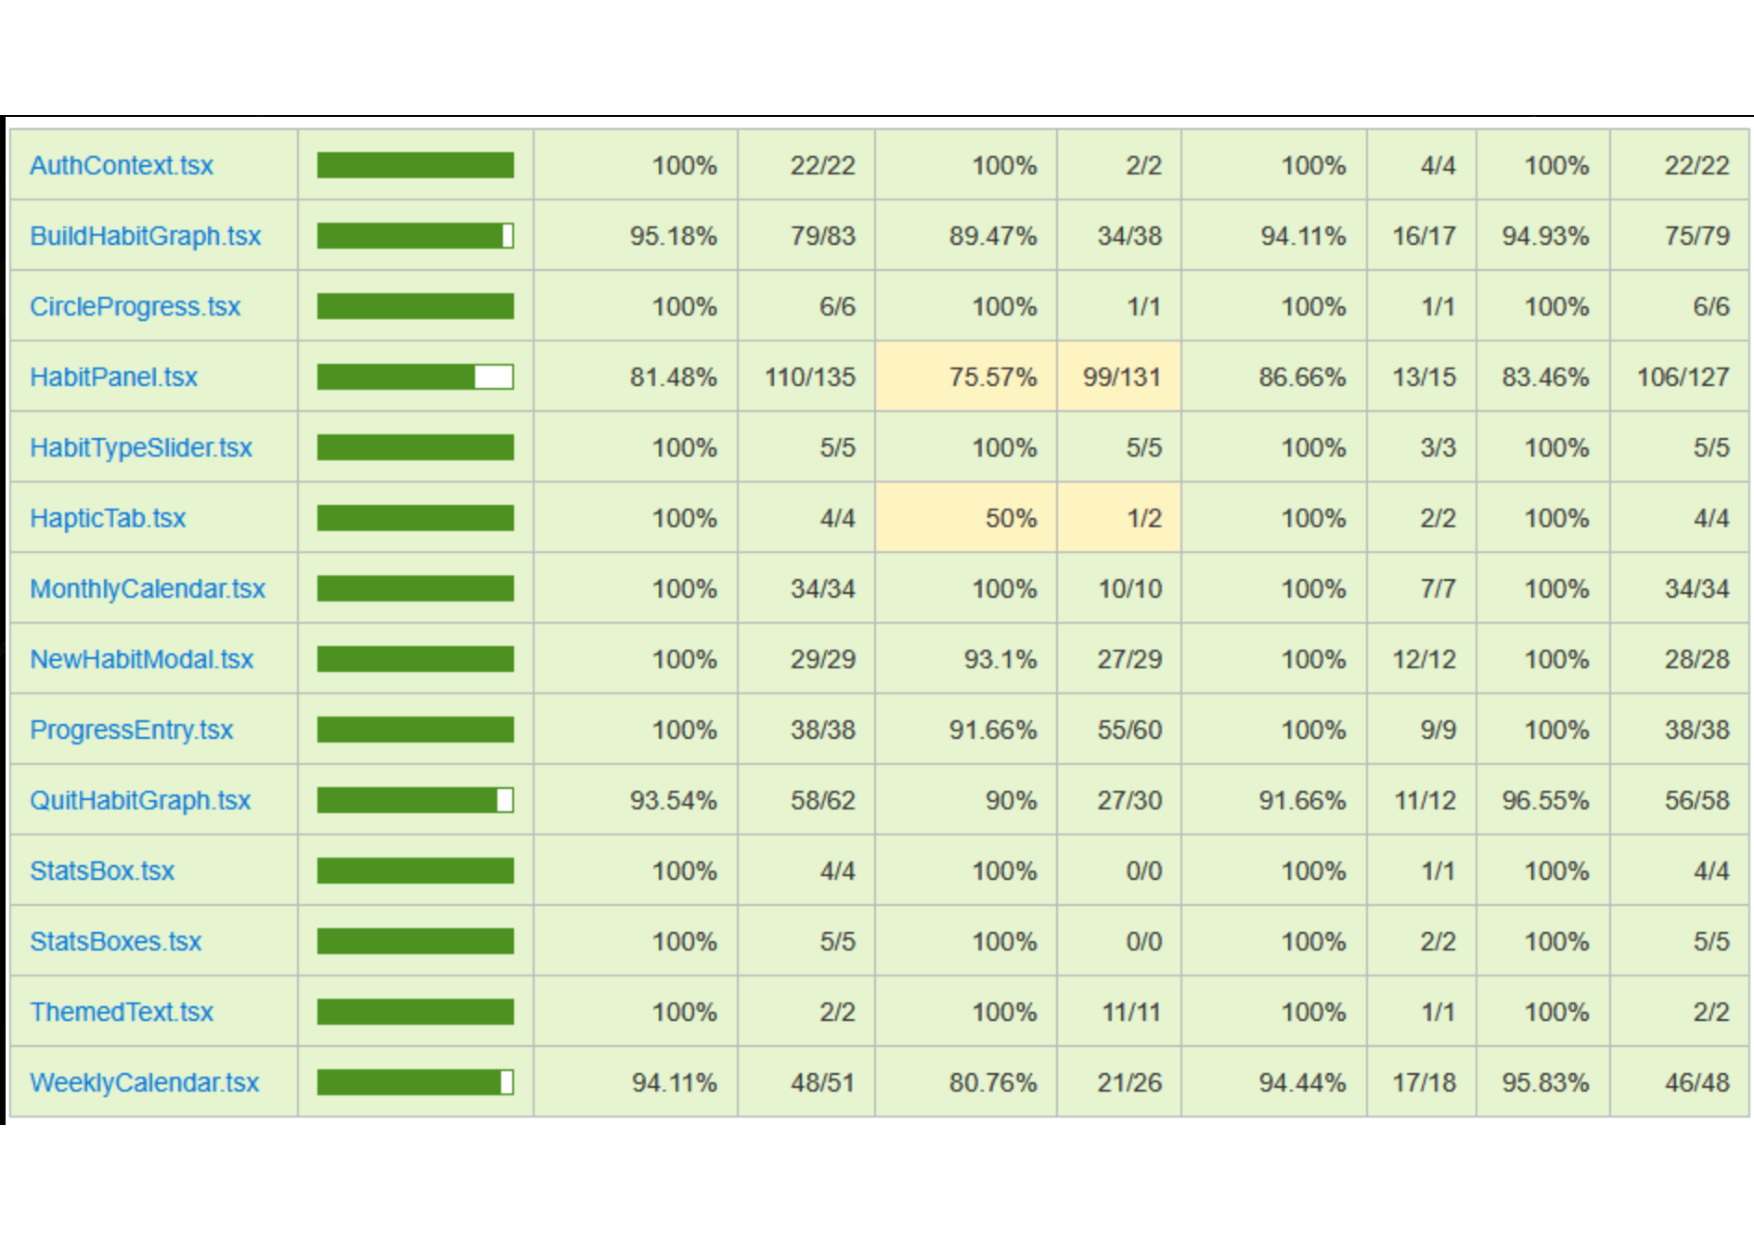
\includegraphics[width=0.8\textwidth]{resources/test_one.pdf}
    \caption{Test Coverage Report for client-side}
    \label{fig:test_one}
\end{figure}

\subsection{Test Coverage Report} \label{sect:test-coverage} 
\begin{figure}[H]
    \centering
    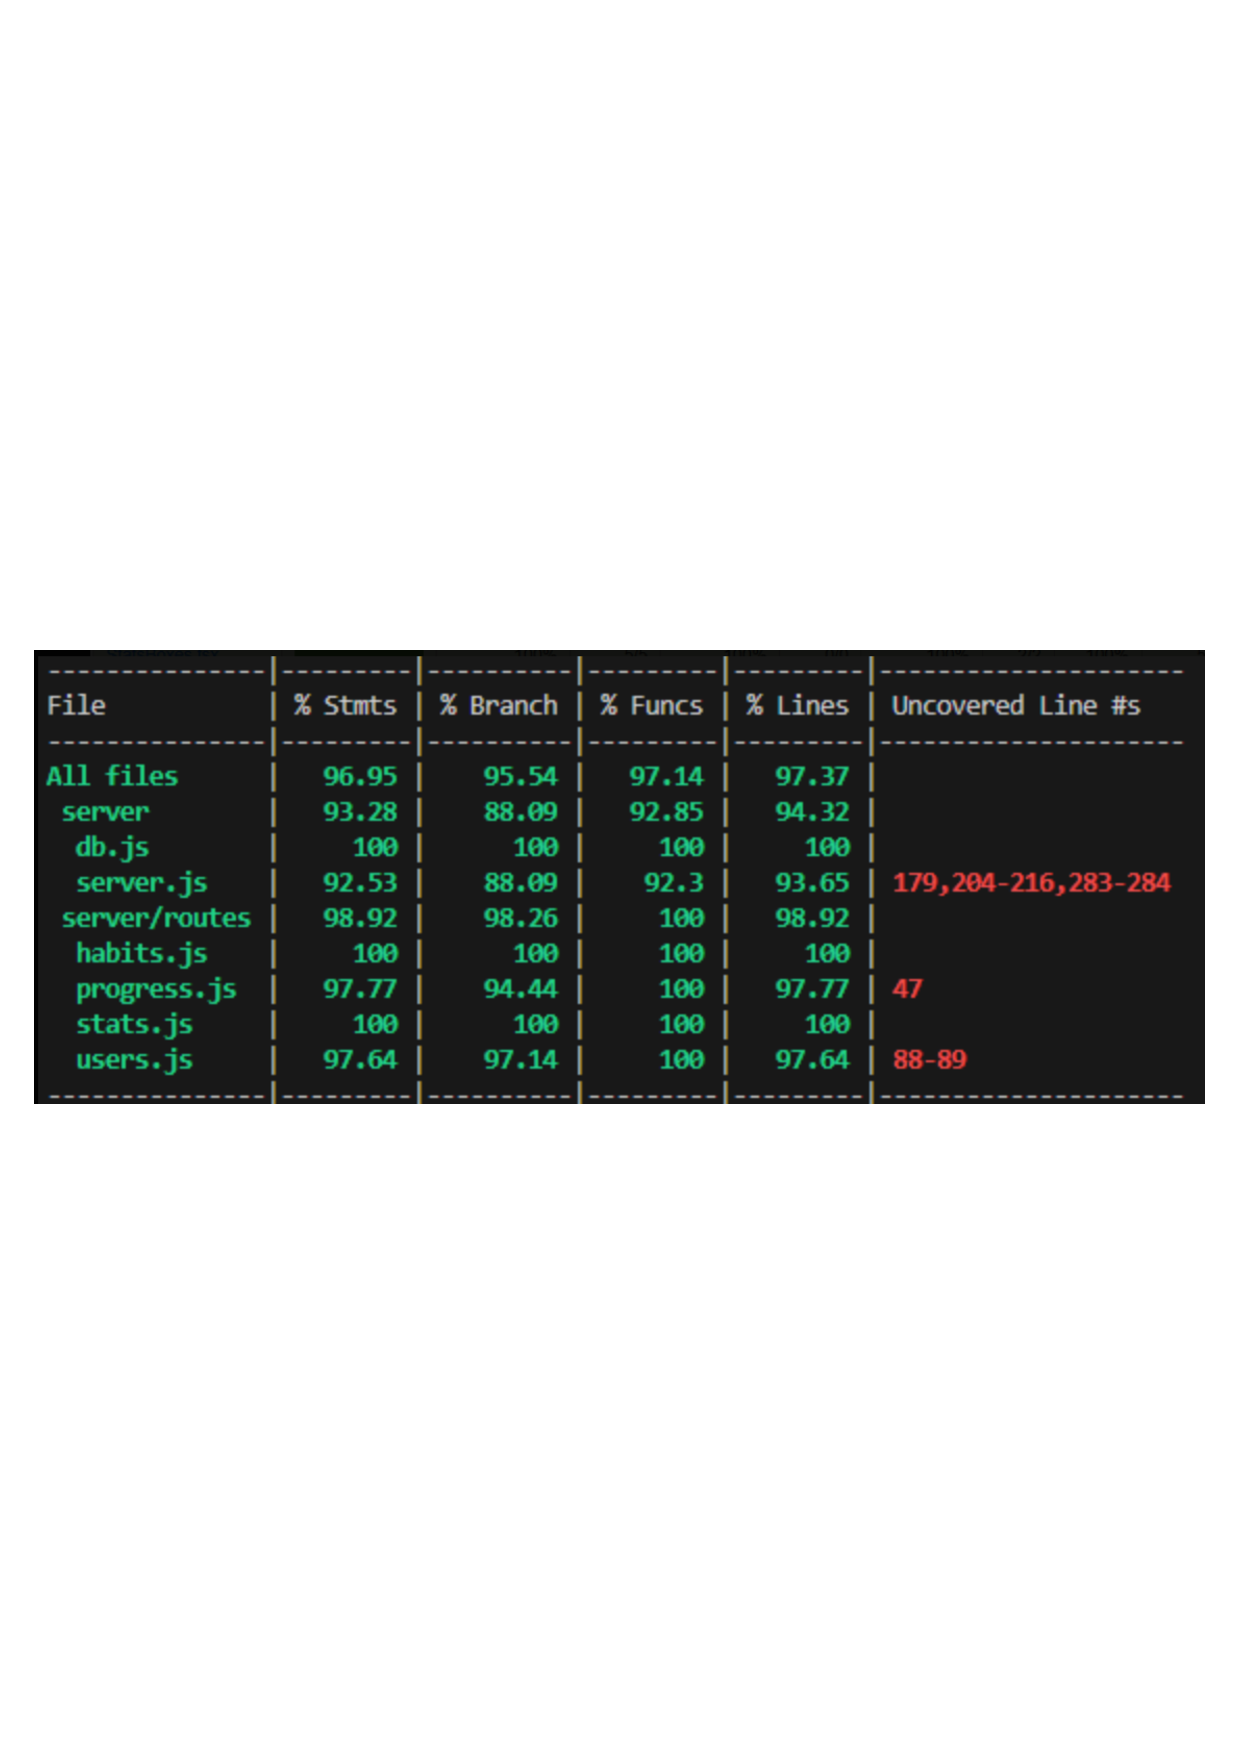
\includegraphics[width=0.8\textwidth]{resources/test_two.pdf}
    \caption{Test Coverage Report for server-side}
    \label{fig:test_two}
\end{figure}

\subsection{Test Coverage Report} \label{sect:test-coverage} 
\begin{figure}[H]
    \centering
    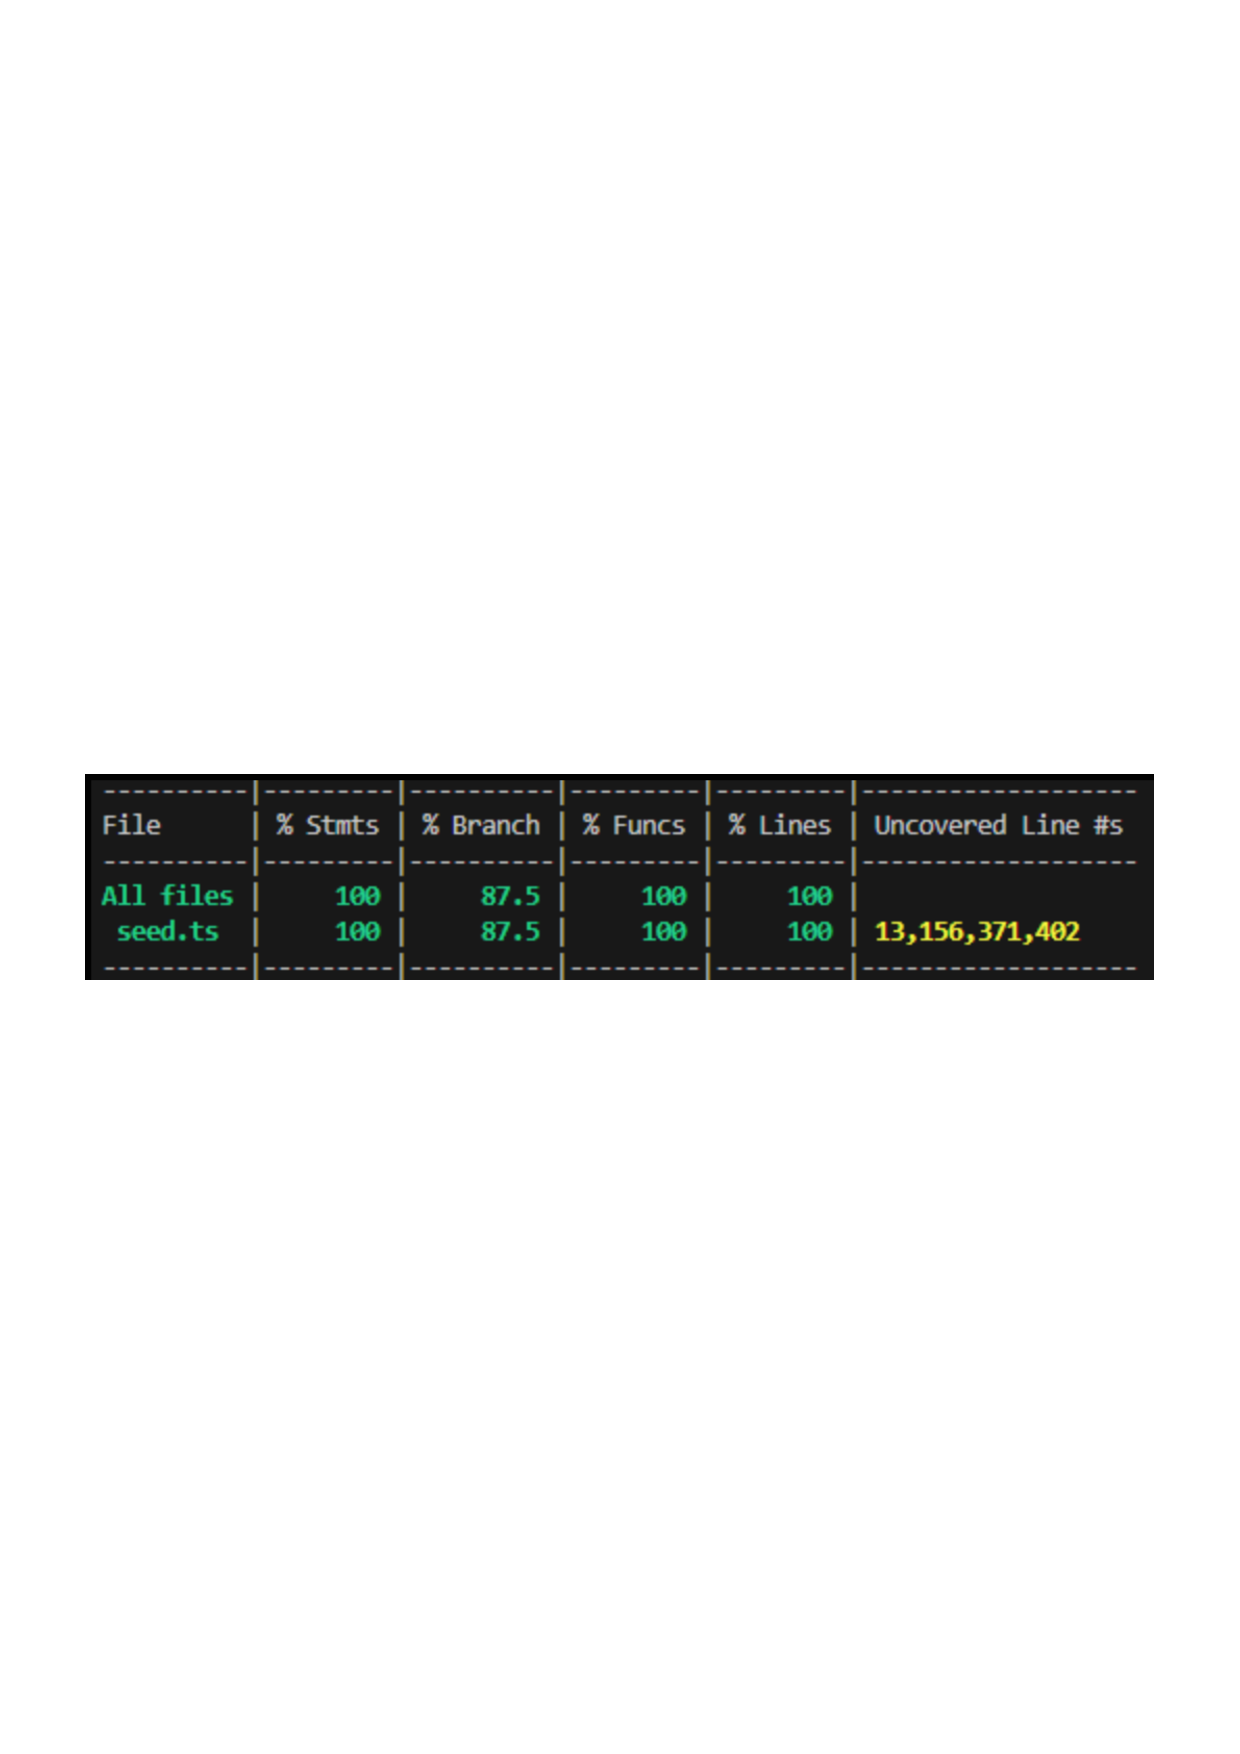
\includegraphics[width=0.8\textwidth]{resources/test_three.pdf}
    \caption{Test Coverage Report}
    \label{fig:test_three}
\end{figure}

Figure \ref{fig:test_one}, \ref{fig:test_two}, and \ref{fig:test_three} shows our test coverage reports. The source coverage details (HTML pages) are located in the project’s coverage/lcov-report folder, particularly in the index.html file. 


\section{Evaluation of testing} \label{sect:testing:evaluation}

\subsection{Strengths} \begin{itemize} \item \textbf{Extensive Automated Coverage}: Our Jest tests are well-integrated, ensuring we can trust most core functionalities. Mocking external dependencies (network, storage, theming) keeps our tests deterministic and easier to maintain. \item \textbf{UI Testing}: By using React Native Testing Library, we test not just logic but actual user interactions (tapping buttons, text input, etc.). \item \textbf{Cross-Platform Verification}: Manual checks on iOS, Android, and web prevent platform-specific issues and ensures a consistent experience. \end{itemize}

\subsection{Weaknesses and Reflections} \begin{itemize} \item \textbf{Fewer Formal Inspections}: We relied heavily on automation due to limited time. This left less room for structured peer review or code inspection, which can catch architecture-level or readability issues that tests may miss. \item \textbf{Lack of External Black-Box Testing}: Although we occasionally showed demos to family/friends, we did not organise a broader group of external testers. This might have revealed usability issues or inconsistencies that a developer-focused approach could overlook.\end{itemize}

\subsection{Future Improvements} \begin{itemize} \item \textbf{More Peer Reviews}: In future we would review each other’s pull requests more often and thoroughly, which could reduce hidden defects early on. \item \textbf{Black-Box Testing:} Bringing in more people who haven’t seen our code would provide fresh perspectives and more thorough user feedback. \item \textbf{Formalising Manual Test Cases}: Storing each manual test case (actions, expected results) in a shared document would add clarity and accountability for each test run.
\item \textbf{Automated Testing during Development}: We would prioritise the need test more thoroughly throughout the entire project, making sure no functionalities were left untested for longer than necessary.\end{itemize}

\noindent Overall, our mix of automated tests and manual checks gave us confidence in our software’s correctness and stability. However, we recognise that further improvements could be made to our testing to strengthen our quality assurance.